\documentclass{josis}

\usepackage{comment}
\usepackage{hyperref}
\usepackage[hyphenbreaks]{breakurl}
\usepackage{booktabs}
\usepackage{stmaryrd}
\usepackage[T1]{fontenc}
\usepackage{cite}
\usepackage{subcaption}

\usepackage{algorithm}
\usepackage{algpseudocode}
\usepackage{pythonhighlight}

\usepackage{amssymb,amsmath}
\usepackage{lastpage}

\begin{document}

\renewcommand{\topfraction}{0.9} 
\renewcommand{\textfraction}{0.1}

\sloppy
\widowpenalty=10000
\clubpenalty=10000
\hyphenpenalty=75

\josisdetails{%
   Team=4, year=2024, firstpage=1, lastpage=\pageref{LastPage}, 
  doi={IUCP-2024},
  }

\urlstyle{rm}
\makeatletter
\let\UrlSpecialsOld\UrlSpecials
\def\UrlSpecials{\UrlSpecialsOld\do\/{\Url@slash}\do\_{\Url@underscore}}%
\def\Url@slash{\@ifnextchar/{\kern-.11em\mathchar47\kern-.2em}%
    {\kern-.0em\mathchar47\kern-.08em\penalty\UrlBigBreakPenalty}}
\def\Url@underscore{\nfss@text{\leavevmode \kern.06em\vbox{\hrule\@width.3em}}}
\makeatother

\hypersetup{
colorlinks=true,
linkcolor=black,
citecolor=black,
urlcolor=black
} 

\runningauthor{\begin{minipage}{.9\textwidth}\centering Rahul Biju, Kevin Thomas, Jobinjoy Ponnappal\end{minipage}}
\runningtitle{Rainfall Prediction}

\title{Rainfall Prediction Using Python and Machine Learning}

\author{Rahul Biju}
\author{Kevin Thomas }
\author{Jobinjoy Ponnappal}\affil{Saintgits Group of Institutions, Kottayam, Kerala}
\date{}

\maketitle

% Add your content here



\maketitle
% Add 5-10 keywords for every submission
\keywords{rainfall prediction, machine learning, Australia, meteorological data, weather stations, data preprocessing, feature selection, Random Forest, accuracy, ROC AUC, agriculture, and disaster preparedness.}
% Add a short abstract of 150-250 words 
\begin{abstract}
This study investigates rainfall prediction in Australia using machine learning techniques. The problem entails predicting whether it will rain the next day based on meteorological data collected over a ten-year period from various weather stations across the country. The methodology involves data exploration, preprocessing, feature selection, and model training using six different algorithms. The study demonstrates the potential of machine learning in improving rainfall prediction accuracy, with implications for sectors such as agriculture and disaster preparedness. 
\end{abstract}
% Your main text begins here. 
\section{Introduction}
Accurate rainfall prediction is crucial for agriculture, disaster management, and water resource planning, particularly in countries like Australia where climate variability poses significant challenges. Despite advancements in meteorological science, accurately forecasting rainfall remains complex due to weather pattern variability. Machine learning offers promise in improving accuracy by leveraging historical meteorological data. This project aims to develop a rainfall prediction model for Australia using machine learning algorithms. The significance lies in its potential to provide insights into future rainfall patterns, enabling informed decision-making in agriculture and disaster preparedness. The primary objective is to develop a machine learning model that accurately predicts rainfall in different Australian regions. By analyzing historical data and employing advanced techniques, the model seeks to enhance existing prediction methods and improve agricultural resilience and disaster management strategies.

\section{Literature Review}
Researchers have explored various techniques for rainfall prediction, aiming for enhanced accuracy across different regions. Parmar and Mistree [9] found that artificial neural network (ANN) models, particularly error back propagation (EBP), offer superior accuracy compared to traditional statistical methods, with ANN outperforming other techniques like ARIMA, SVM, and SOM. Barrera-Animas et al. [2] demonstrated that Bidirectional-LSTM and Stacked-LSTM models exhibit superior performance for rainfall forecasting, although challenges such as overfitting persist, suggesting the need for parameter fine-tuning and exploration of alternative approaches. Cramer et al. [5] evaluated methods for predicting accumulated rainfall using a sliding window approach and various machine learning algorithms, while Atta-ur Rahman et al. [10] implemented classification techniques on real-time rainfall data from Lahore. Mohammed et al. [8] analyzed a Lahore rainfall dataset using multiple regression methods, with Support Vector Regression (SVR) showing the highest accuracy. Furthermore, Appiah-Badu et al. [1] contributed to rainfall prediction by employing classification algorithms on Ghanaian climatic data spanning 1980 to 2019, across different ecological zones.

\section{Methodology}
During the training of the rainfall prediction model, various machine learning algorithms were employed, including Logistic Regression, Decision Tree, Random Forest, Light GBM, Catboost, and XGBoost. The dataset used for model training was collected from Kaggle, a prominent platform for sharing and discovering datasets. Various stages in the implementation process included:
\begin{description}
\textbf{Pre-processing \& Data cleaning:} The initial step involves cleaning and preparing the loaded data to make it suitable for utilization with machine learning algorithms.
Data cleaning techniques are applied to handle missing values, outliers, and any inconsistencies in the dataset.
\newline
\textbf{Feature extraction:} Feature extraction is the method of converting raw data into meaningful features suitable for input into machine learning algorithms. In the program, feature extraction is specifically conducted to derive the binary representations of the features "RainToday" and "RainTomorrow".
\newline
\textbf{Feature selection:} Feature importance is assessed using various techniques to identify the most relevant features for training the model.The filter (chi-square value) and wrapper (Random Forest) methods are implemented for feature selection to enhance model performance.
Filter methods evaluate the statistical significance of each feature independently, while wrapper methods assess the collective importance of features through iterative model training.
The selected features are retained for subsequent model training, ensuring that only the most informative attributes are utilized.
\newline
\textbf{Data Splitting:} Following feature extraction, the dataset is divided into separate training and testing sets.
This partitioning facilitates the training of the machine learning models on one subset of data while evaluating their performance on an independent subset.
Common splitting ratios, such as 75\% for training and 25\% for testing, are often employed to ensure an adequate balance between model training and evaluation.
\newline
    %\item[Classification:] Implementing various Machine Learning Classification models on the document matrix to classify the input text into fake or true news.
\textbf{Model Training:} Various machine learning algorithms, including Logistic Regression, Decision Tree, Random Forest, Light GBM, Catboost, and XGBoost are employed to train the rainfall prediction model. Each algorithm learns patterns and relationships from the training data to make predictions about future rainfall occurrences.
    Logistic Regression is a linear model used for binary classification, predicting the probability of a certain outcome based on input features. Decision Trees recursively partition the feature space into regions, making decisions based on simple if-else conditions. Random Forests combine multiple decision trees to improve predictive accuracy and reduce overfitting. Light GBM is a gradient boosting framework known for its speed and efficiency, achieved through a novel tree-growing algorithm. Catboost is a gradient boosting library that efficiently handles categorical variables, using specialized techniques to optimize performance. XGBoost is a powerful gradient boosting library optimized for speed and scalability on structured data, offering high performance across various applications. 
\newline
\textbf{Model Evaluation and Selection:} Trained models undergo comprehensive evaluation using various performance metrics, including Accuracy, Precision, Recall, F1 Score, ROC Curve, AUC-ROC, and Confusion Matrix. This evaluation identifies strengths and weaknesses, guiding the selection of the most suitable algorithm for rainfall prediction. The best-performing model is chosen based on this analysis and reported transparently, with associated performance metrics. Insights gained may inform further refinements before deployment.
\newline
\text{Accuracy} = (\text{Correct Predictions} / \text{Total Predictions}) \times 100\%
\newline
\text{Precision} = \text{True Positives}/(\text{True Positives} + \text{False Positives})
\newline
\text{Recall} = \text{True Positives}(\text{True Positives} + \text{False Negatives})
\newline
\text{F1 Score} = 2 \times \frac{\text{Precision} \times \text{Recall}}{\text{Precision} + \text{Recall}}

\end{description} 
\section{Implementation}
As the first step in the task, the file containing the dataset [4] is loaded. The dataset comprises weather-related attributes such as date, location, temperature (minimum and maximum), rainfall, evaporation, sunshine duration, wind direction and speed, humidity levels, atmospheric pressure, cloud cover, and rain occurrence. Figure\ref{fig:subfig1} illustrates the presence of non-binary data points. To align with computational standards, the target variable ("RainTomorrow"), which are objects, needs to be converted into binary.


\begin{figure}[!h]
    \centering
    
    \begin{subfigure}[b]{0.4\textwidth}
        \centering
        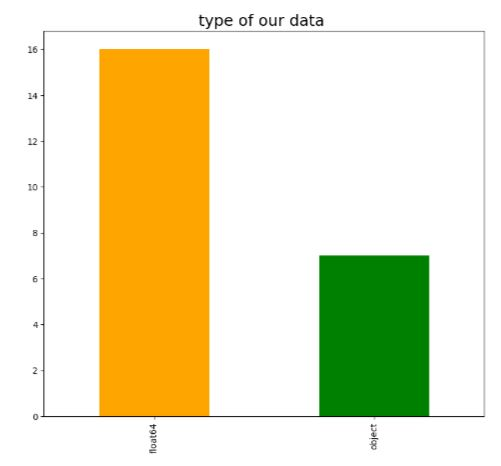
\includegraphics[width=\textwidth]{bargraph of data type.JPG}
        \caption{Type of data}
        \label{fig:subfig1}
    \end{subfigure}
    \hfill
    \begin{subfigure}[b]{0.4\textwidth}
        \centering
        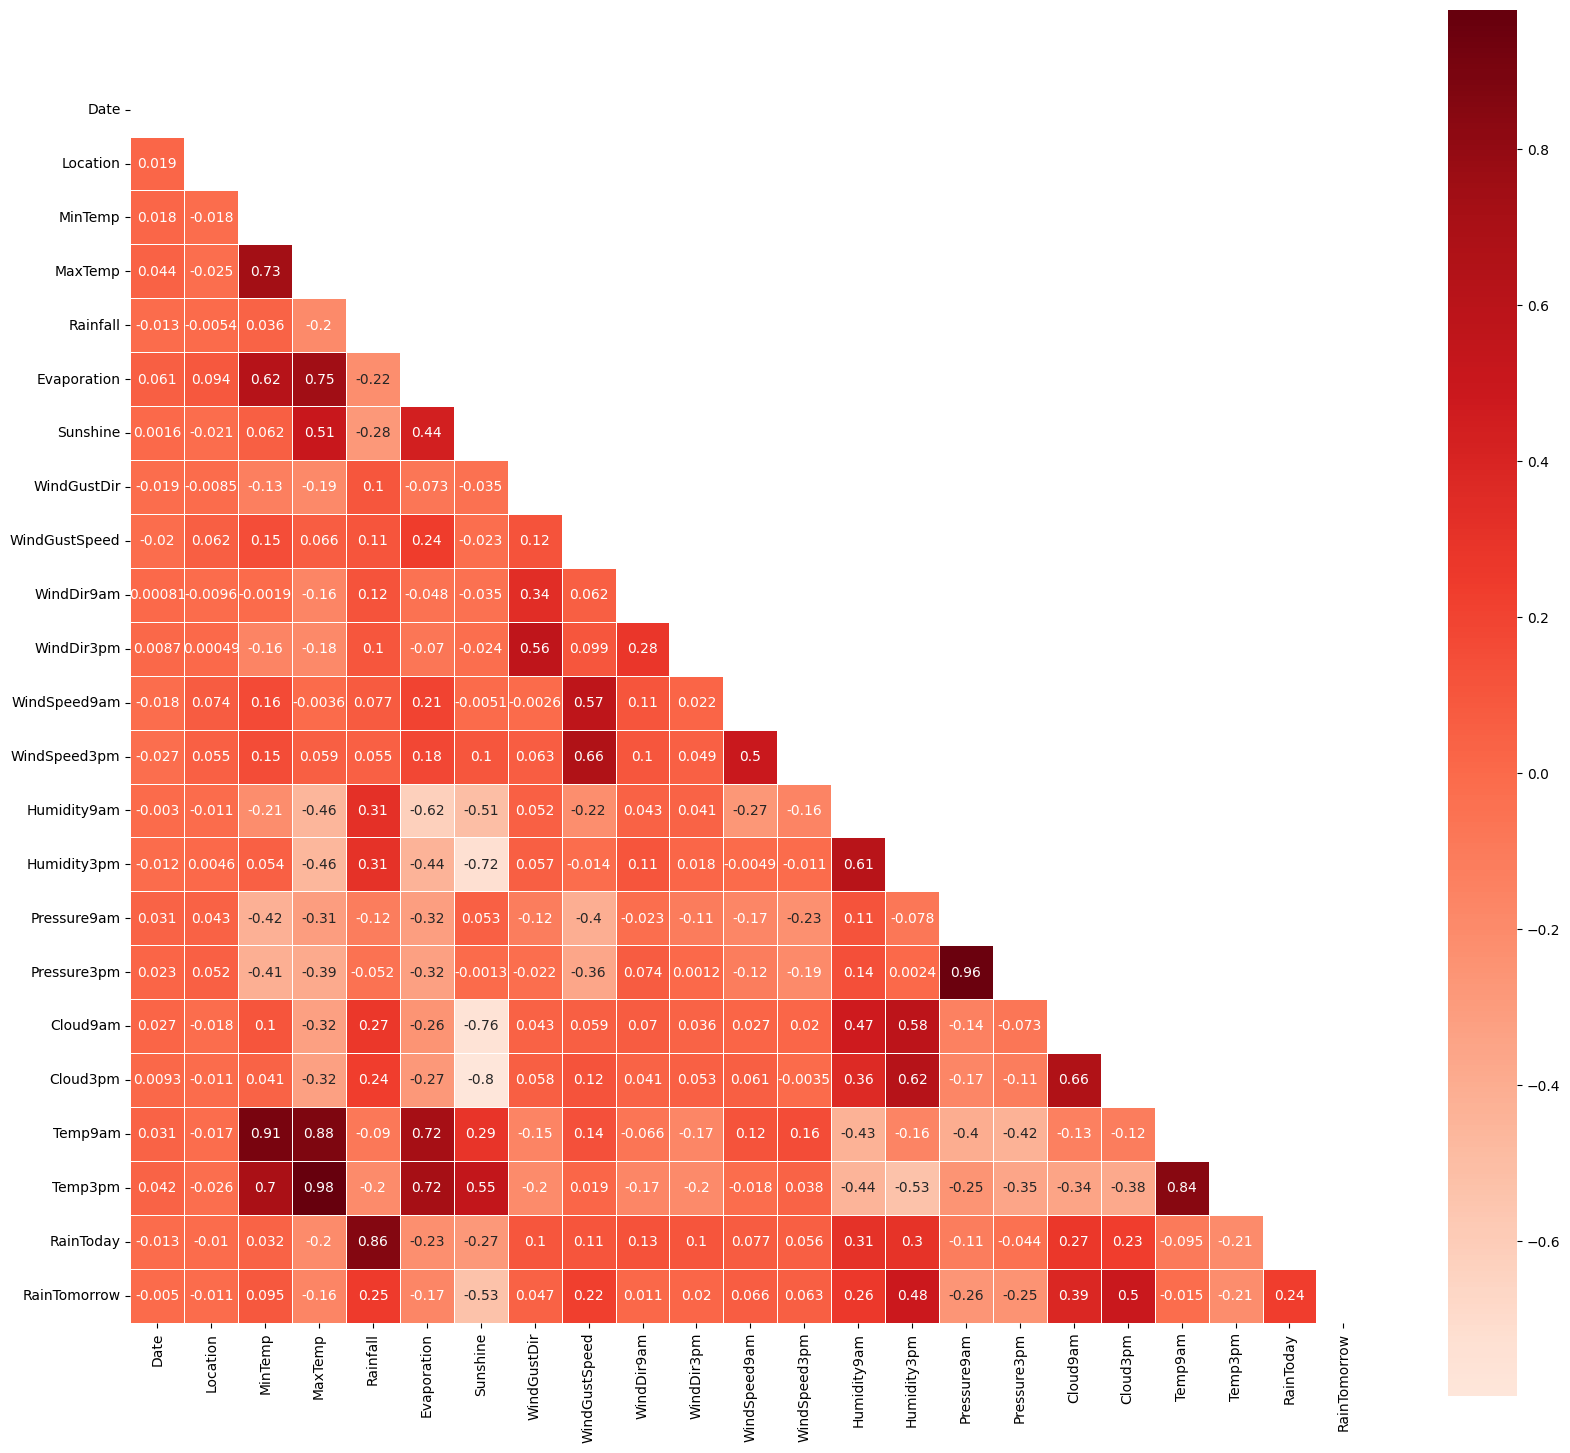
\includegraphics[width=\textwidth]{correlation.JPG}
        \caption{Heat Map}
        \label{fig:subfig2}
    \end{subfigure}
    
    \caption{Data Visualisation}
    \label{fig:mainfig}
\end{figure}

The analysis of the target variable ("RainTomorrow") reveals a class imbalance. The data exhibits a 78:22 ratio for "No Rain" (class 0) and "Rain" (class 1) occurrences, respectively.The class imbalance in the target variable ("RainTomorrow") can affect the dataset by biasing the machine learning model towards the majority class ("No Rain"). This imbalance may result in the model having reduced predictive accuracy for the minority class ("Rain") as it receives less emphasis during training.  To address this imbalance and improve model performance, the data will be pre-processed, creating a more balanced dataset for training the machine learning model.
The pre-processing and cleaning stage is completed in the following way:

To address class imbalance where "Rain" is the minority class, oversampling "Rain" instances or using SMOTE to generate synthetic minority class data are potential approaches. Data preprocessing steps like imputation (mode for categorical, MICE for numerical) and transformation (label encoding for categorical variables) can be applied. Additionally, outliers are identified using IQR and removed or transformed. 

Observing that the original dataset had the form (87927, 24), after removing outliers, the dataset now has the form (86065, 24). Consequently, the dataset is now free of 1862 outliers.
The correlation heat-map is generated to visualize the pairwise correlations between variables in the modified dataset as shown in Figure \ref{fig:subfig2}.


The integration of both filter and wrapper methods for feature selection is seamless. Before initiating feature selection using the chi-square value-based filtering method, normalization of the dataset is imperative. The deliberate selection of MinMaxScaler over StandardScaler ensures the prevention of negative values and strengthens the preprocessing phase for a more robust analysis. Notably, the wrapper method employs Random Forest.
The dataset will be partitioned into training (75\%) and test (25\%) sets for the rainfall prediction model. The rainfall prediction model is trained using a variety of machine learning algorithms, encompassing Logistic Regression, Decision Tree, Random Forest, Light GBM, Catboost, and XGBoost.
\\

\section{Results \& Discussion}

Summary of the results is shown in Table \refTable \ref{tab:large-model} presents the performance of various machine learning models in predicting rainfall data, including their root mean square error (RMSE) value, precision, accuracy, recall, F1-score, and processing time.
\begin{table}%[htp]
\centering
\caption{ Performance of Machine Learning Models in predicting the rainfall data }
\label{tab:large-model}
\begin{tabular}{|c|l|c|c|c|c|c|l|}
\hline
\begin{tabular}[c]{@{}c@{}}Model\\ No.\end{tabular} & \multicolumn{1}{c|}{Model Name} & \begin{tabular}[c]{@{}c@{}}RMSE\\ value\end{tabular} & Precision & Accuracy & Recall & f1-score & \multicolumn{1}{c|}{\begin{tabular}[c]{@{}c@{}}Processing\\ Time\end{tabular}} \\ \hline


1. & Logistic Regression & 0.20 & 0.80 & 0.79 & 0.83 & 0.82 & 1.99s \\ \hline
2. & Decision tree & 0.14 & 0.89 & 0.858 & 0.86 & 0.87 & 0.35s \\ \hline
3. & Random Forest & 0.07 & 0.95 & 0.926 & 0.93 & 0.93 & 21.45s \\ \hline 
4. & Light GBM & 0.13 & 0.87 & 0.866 & 0.886 & 0.88 & 1.265s \\ \hline
5. & Catboost & 0.06 & 0.97 & 0.94 & 0.969 & 0.94 & 99.867s \\ \hline 
6. & XGBoost & 0.05 & 0.98 & 0.95 & 0.976 & 0.95 & 44.945s \\ \hline 
\end{tabular}
\end{table}

The results indicate that ensemble methods such as Random Forest, Light GBM, Catboost, and XGBoost outperform traditional models like Logistic Regression and Decision Tree. Catboost and XGBoost achieved the highest precision, accuracy, recall, and F1-score, indicating their superior performance in predicting rainfall occurrences. However, they also require longer processing times compared to other models, especially Catboost with a processing time of 99.867 seconds.

These findings contribute significantly to addressing the problem identified in the introduction by providing a clear understanding of the effectiveness of different machine learning algorithms in rainfall prediction. The high accuracy and precision of models like Catboost and XGBoost demonstrate their potential to improve weather forecasting accuracy, which is crucial for various sectors such as agriculture, disaster management, and infrastructure planning. Additionally, the relatively low processing time of models like Decision Tree and Logistic Regression makes them suitable for real-time applications where speed is essential.

Overall, the results underscore the importance of selecting appropriate machine learning algorithms for rainfall prediction tasks and provide valuable insights for stakeholders to make informed decisions in mitigating the risks associated with extreme weather events.

The ROC Curve and Confusion matrix for each model is given in figures \ref{FIGURE LABEL1},\ref{FIGURE LABEL2} and \ref{FIGURE LABEL3}.

\begin{figure}[!h]%[H]
\centering
\begin{subfigure}{.24\textwidth}
    \centering
    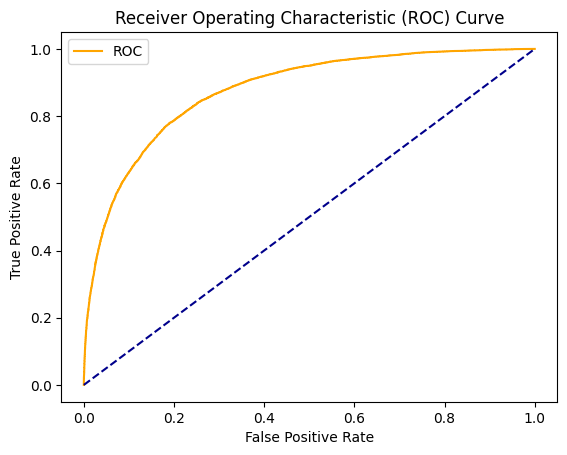
\includegraphics[width=0.95\linewidth]{ROC1.png}  
    \caption{i}
    \label{SUBFIGURE LABEL 1}
\end{subfigure}
\begin{subfigure}{.24\textwidth}
    \centering
    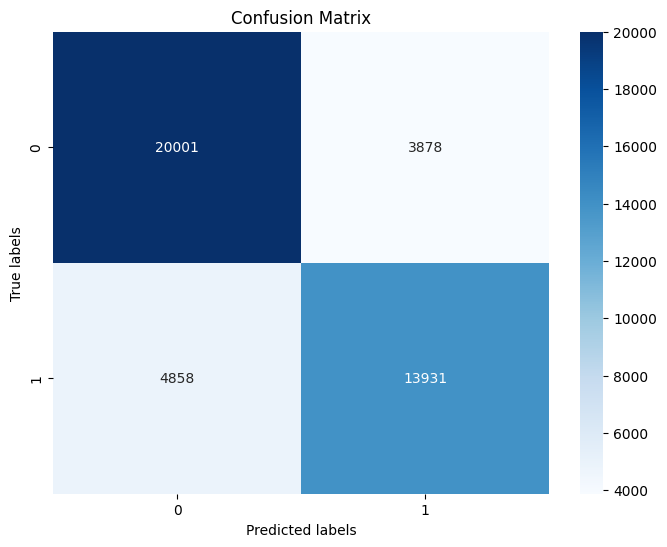
\includegraphics[width=0.95\linewidth]{CM1.png}  
    \caption{i}
    \label{SUBFIGURE LABEL 2}
\end{subfigure}
\begin{subfigure}{.24\textwidth}
    \centering
    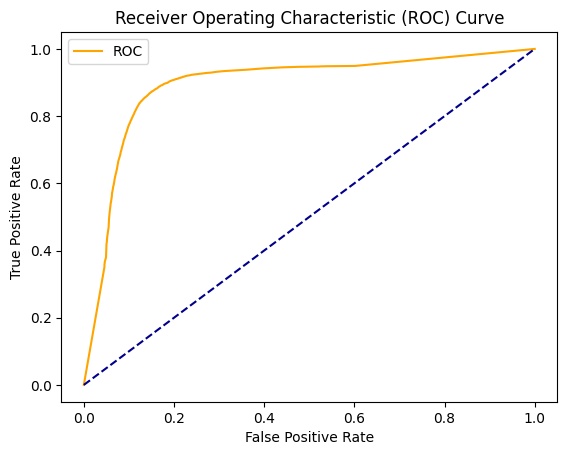
\includegraphics[width=0.95\linewidth]{ROC2.png}  
    \caption{ii}
    \label{SUBFIGURE LABEL 3}
\end{subfigure}
\begin{subfigure}{.24\textwidth}
    \centering
    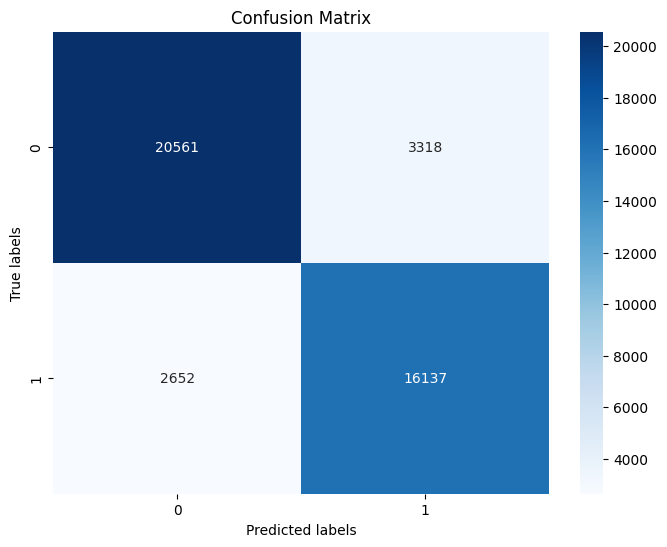
\includegraphics[width=0.95\linewidth]{CM2.png}  
    \caption{ii}
    \label{SUBFIGURE LABEL 4}
\end{subfigure}
\caption{(i) Logistic Regression and (ii) Decision Tree}
\label{FIGURE LABEL1}
\end{figure}

\begin{figure}
\centering


\begin{subfigure}{.24\textwidth}
    \centering
    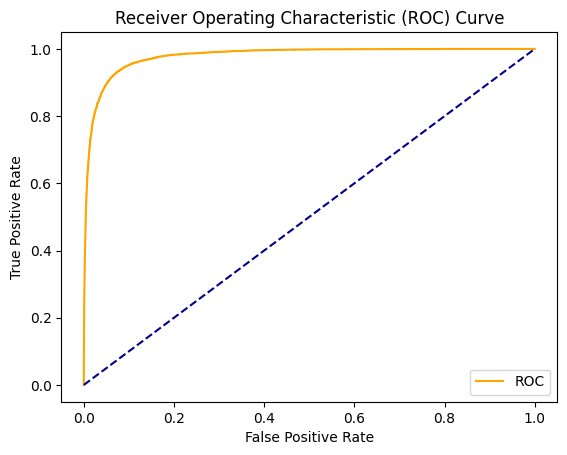
\includegraphics[width=0.95\linewidth]{ROC3.png}  
    \caption{i}
    \label{SUBFIGURE LABEL 1}
\end{subfigure}
\begin{subfigure}{.24\textwidth}
    \centering
    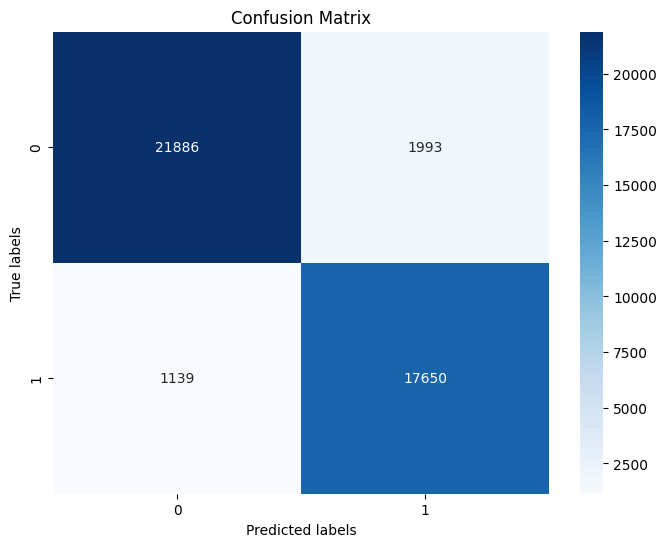
\includegraphics[width=0.95\linewidth]{CM3.png}  
    \caption{i}
    \label{SUBFIGURE LABEL 2}
\end{subfigure}
\begin{subfigure}{.24\textwidth}
    \centering
    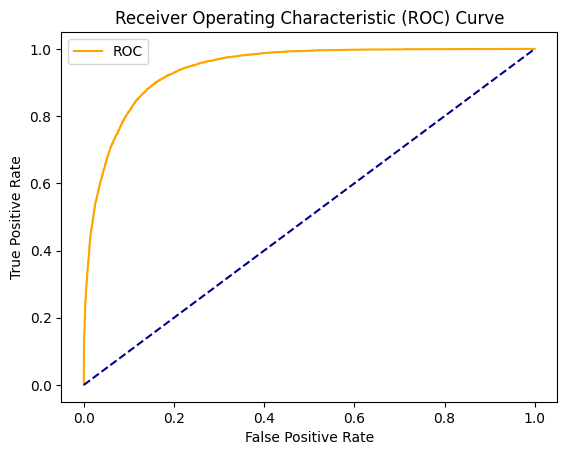
\includegraphics[width=0.95\linewidth]{ROC4.png}  
    \caption{ii}
    \label{SUBFIGURE LABEL 3}
\end{subfigure}
\begin{subfigure}{.24\textwidth}
    \centering
    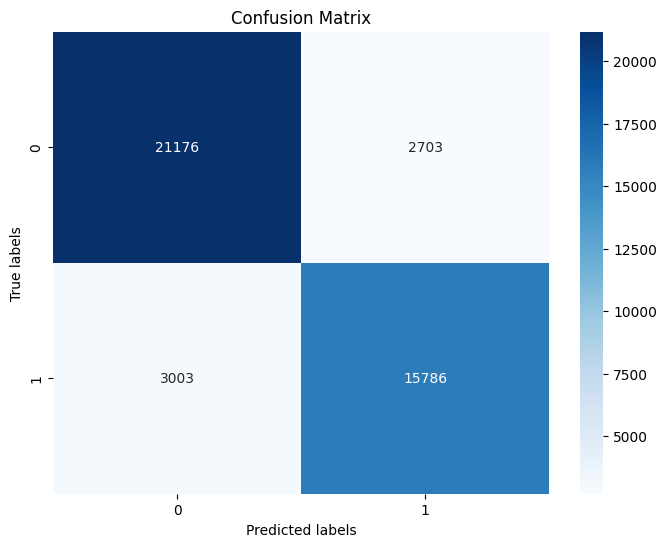
\includegraphics[width=0.95\linewidth]{CM4.png}  
    \caption{ii}
    \label{SUBFIGURE LABEL 4}
\end{subfigure}
\caption{(i) Random Forest and (ii) Light GBM}
\label{FIGURE LABEL2}
\end{figure}

\begin{figure}[!h]%[H]
\centering


\begin{subfigure}{.24\textwidth}
    \centering
    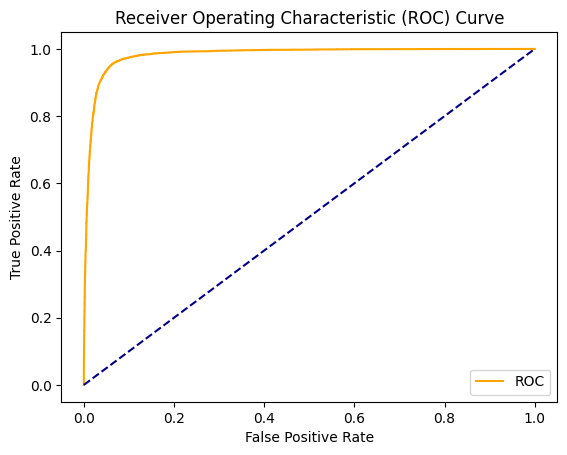
\includegraphics[width=0.95\linewidth]{ROC5.png}  
    \caption{i}
    \label{SUBFIGURE LABEL 1}
\end{subfigure}
\begin{subfigure}{.24\textwidth}
    \centering
    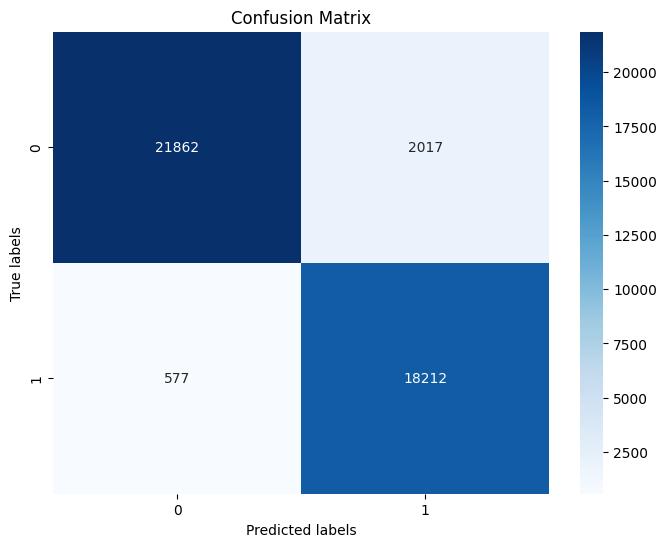
\includegraphics[width=0.95\linewidth]{CM5.png}  
    \caption{i}
    \label{SUBFIGURE LABEL 2}
\end{subfigure}
\begin{subfigure}{.24\textwidth}
    \centering
    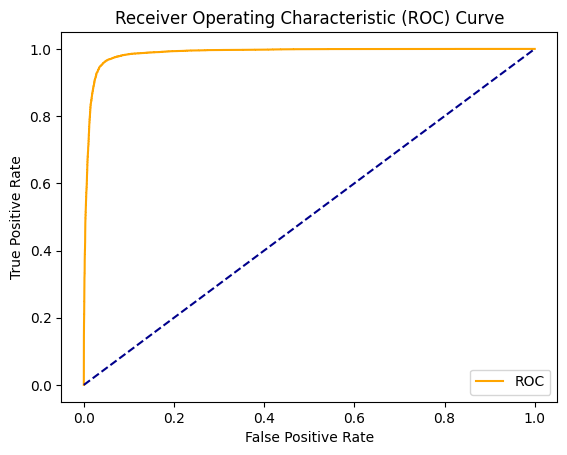
\includegraphics[width=0.95\linewidth]{ROC6.png}  
    \caption{ii}
    \label{SUBFIGURE LABEL 3}
\end{subfigure}
\begin{subfigure}{.24\textwidth}
    \centering
    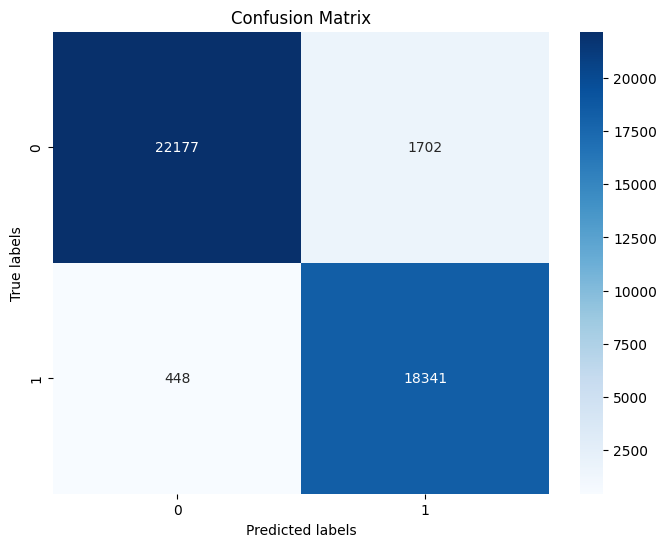
\includegraphics[width=0.95\linewidth]{CM6.png}  
    \caption{ii}
    \label{SUBFIGURE LABEL 4}
\end{subfigure}
\caption{(i) Catboost and (ii) XGBoost}
\label{FIGURE LABEL3}
\end{figure}


\section{Conclusions}
In conclusion, the study evaluated various machine learning algorithms for rainfall prediction using historical meteorological data from Kaggle. Ensemble methods like Catboost and XGBoost outperformed traditional models such as Logistic Regression and Decision Tree, achieving higher precision, accuracy, recall, and F1-score. Although Catboost and XGBoost had longer processing times, their superior performance makes them valuable for accurate rainfall forecasting, benefiting sectors like agriculture and disaster management.

The significance of the findings lies in their potential to improve weather forecasting accuracy, thereby aiding in disaster preparedness, resource allocation, and infrastructure planning. The study underscores the importance of selecting appropriate machine learning algorithms for specific prediction tasks and highlights the trade-offs between accuracy and processing time.

For future research, investigating methods to optimize the processing time of high-performing models like Catboost and XGBoost would be beneficial. Additionally, exploring ensemble techniques or hybrid models that combine the strengths of different algorithms could further enhance prediction accuracy.

In practical applications, stakeholders should consider the trade-offs between model performance and computational resources when selecting a suitable algorithm for rainfall prediction. Moreover, integrating real-time data sources and enhancing model interpretability could enhance the usability and reliability of rainfall prediction systems in various sectors.

Overall, the study provides valuable insights into the application of machine learning for rainfall prediction, offering practical implications for decision-makers and researchers alike.

\section*{Acknowledgments}
We are deeply grateful to Intel® Corporation for the opportunity afforded to us in this project. Our heartfelt appreciation goes to our esteemed team mentor, Gayathri J L, for her invaluable counsel and unwavering backing throughout the project's duration. Saintgits College of Engineering and Technology deserves our thanks for equipping us with the requisite resources and conducting enlightening sessions on machine learning. We extend our gratitude to the experts in the realms of machine learning and artificial intelligence, whose groundbreaking contributions have paved the way for our project. We also recognize the mentors for their indispensable guidance and encouragement during our participation in the Intel® - Unnati Programme. Their expertise and motivation have been pivotal in shaping our project.

\cite{*}
\bibliographystyle{josisacm}
\bibliography{josisexample}
\appendix


\section{Appendix}

\subsection{Loading data from the source}
Data for this project is taken from the source: \url{https://www.kaggle.com/datasets/jsphyg/weather-dataset-rattle-package/download?datasetVersionNumber=2}.

The python code section for this stage is shown bellow:
\begin{python}
import requests

# File share link
file_url = "https://drive.google.com/uc?export=download&id=1t2K281W4paE1gOuFtJUHmbc4iKcWiULb"

# Path where you want to save the file in Colab
save_path = "Weather_DataSet.csv"

# Send a GET request to the file URL
response = requests.get(file_url)

# Check if the request was successful (status code 200)
if response.status_code == 200:
    # Write the content of the response to a file
    with open(save_path, 'wb') as f:
        f.write(response.content)
    print("File downloaded successfully!")
else:
    print("Failed to download the file. Status code:", response.status_code)
\end{python}

\subsection{Data Exploration}
Data exploration is essential for understanding dataset characteristics and patterns.
\begin{python}
df.shape
df.info()
\end{python}

\subsection{Visualization of Dataset}
Visualization of datasets is crucial for understanding data distributions, patterns, and relationships. 
\begin{python}
import matplotlib.pyplot as plt

fig, axarr = plt.subplots(1, 2, figsize=(20, 8))

df.dtypes.value_counts().plot.pie(explode=[0.1,0.1],autopct='%1.1f%%',shadow=True,ax=axarr[1],colors= ['orange','green'])
axarr[1].set_title("Dataset Division ", fontsize=18)

df.dtypes.value_counts().plot(kind='bar',ax=axarr[0],color= ['orange','green'])
plt.title('Dataset Division');
axarr[0].set_title("type of our data ", fontsize=18)
\end{python}   

\subsection{Data cleaning and pre-processing}
The data pre-processing and cleaning procedures involve handling missing values, class imbalance and addressing outliers to ensure the dataset's quality. Techniques like imputation and transformation are applied to fill in missing data, ensuring the dataset is ready for analysis and modeling.
\begin{python}
# Convertion of RainToday and RainTomorrow which are objects in the
# form of (Yes / No) to binary (1/0).
df['RainToday'].replace({'No': 0, 'Yes': 1},inplace = True)
df['RainTomorrow'].replace({'No': 0, 'Yes': 1},inplace = True)
\end{python}

\begin{python}
# Handling Class Imbalance by OverSampling
from sklearn.utils import resample

no = df[df.RainTomorrow == 0]
yes = df[df.RainTomorrow == 1]
yes_oversampled = resample(yes, replace=True, n_samples=len(no), random_state=123)
oversampled = pd.concat([no, yes_oversampled])

# Plot the distribution after oversampling
fig = plt.figure(figsize=(8, 5))
oversampled['RainTomorrow'].value_counts(normalize=True).plot(kind='bar', color=['orange', 'green'], alpha=0.9, rot=0)
plt.title('RainTomorrow Indicator No(0) and Yes(1) after Oversampling (Balanced Dataset)')
plt.show()
\end{python}

\begin{python}
# Checking for missing datas in Dataset
missing_values=df.isnull().sum() # missing values

percent_missing = df.isnull().sum()/df.shape[0]*100 # missing value %

value = {
    'missing_values ':missing_values,
    'percent_missing %':percent_missing ,
     'data type' : df.dtypes
}
frame=pd.DataFrame(value)
frame
\end{python}

\begin{python}
# Imputation and Transformation
oversampled.select_dtypes(include=['object']).columns

# Impute categorical var with Mode
oversampled['Date'] = oversampled['Date'].fillna(oversampled['Date'].mode()[0])
oversampled['Location'] = oversampled['Location'].fillna(oversampled['Location'].mode()[0])
oversampled['WindGustDir'] = oversampled['WindGustDir'].fillna(oversampled['WindGustDir'].mode()[0])
oversampled['WindDir9am'] = oversampled['WindDir9am'].fillna(oversampled['WindDir9am'].mode()[0])
oversampled['WindDir3pm'] = oversampled['WindDir3pm'].fillna(oversampled['WindDir3pm'].mode()[0])

# Convert categorical features to continuous features with Label Encoding
from sklearn.preprocessing import LabelEncoder
lencoders = {}
for col in oversampled.select_dtypes(include=['object']).columns:
    lencoders[col] = LabelEncoder()
    oversampled[col] = lencoders[col].fit_transform(oversampled[col])
import warnings
warnings.filterwarnings("ignore")

# Multiple Imputation by Chained Equations
from sklearn.experimental import enable_iterative_imputer
from sklearn.impute import IterativeImputer
MiceImputed = oversampled.copy(deep=True)
mice_imputer = IterativeImputer()
MiceImputed.iloc[:, :] = mice_imputer.fit_transform(oversampled)
\end{python}

\begin{python}
# Detecting outliers with IQR
Q1 = MiceImputed.quantile(0.25)
Q3 = MiceImputed.quantile(0.75)
IQR = Q3 - Q1
print(IQR)

# Removing outliers from the dataset
MiceImputed = MiceImputed[~((MiceImputed < (Q1 - 1.5 * IQR)) |(MiceImputed > (Q3 + 1.5 * IQR))).any(axis=1)]
MiceImputed.shape
\end{python}
\subsection{Exploratory data analysis}
Exploratory data analysis involves exploring and understanding the relationships between variables in the dataset before diving into model building.
\begin{python}
# Correlation Heatmap
import numpy as np
import matplotlib.pyplot as plt
import seaborn as sns
corr = MiceImputed.corr()
mask = np.triu(np.ones_like(corr, dtype=bool))
f, ax = plt.subplots(figsize=(20, 20))
cmap = sns.diverging_palette(250, 25, as_cmap=True)
sns.heatmap(corr, mask=mask, cmap='Reds', vmax=None, center=0,square=True, annot=True, linewidths=.5, cbar_kws={"shrink": .9})

# Define a custom color palette
custom_palette = ["green", "orange"]  # Specify colors as needed

# Use pairplot with the custom color palette
sns.pairplot(data=MiceImputed, vars=('MaxTemp','MinTemp','Pressure9am','Pressure3pm', 'Temp9am', 'Temp3pm', 'Evaporation'), hue='RainTomorrow', palette=custom_palette)
\end{python}

\subsection{Feature Selection}
The goal of feature selection is to identify the most relevant and informative features while discarding irrelevant or redundant ones.
\begin{python}
# Standardizing data
from sklearn import preprocessing
r_scaler = preprocessing.MinMaxScaler()
r_scaler.fit(MiceImputed)
modified_data = pd.DataFrame(r_scaler.transform(MiceImputed), index=MiceImputed.index, columns=MiceImputed.columns)
\end{python}
\begin{python}
# Feature Importance using Filter Method (Chi-Square)
from sklearn.feature_selection import SelectKBest, chi2
X = modified_data.loc[:,modified_data.columns!='RainTomorrow']
y = modified_data[['RainTomorrow']]
selector = SelectKBest(chi2, k=10)
selector.fit(X, y)
X_new = selector.transform(X)
print(X.columns[selector.get_support(indices=True)])
\end{python}
\begin{python}
# Selection of features by wrapping method (random forest)
from sklearn.feature_selection import SelectFromModel
from sklearn.ensemble import RandomForestClassifier as rf

X = MiceImputed.drop('RainTomorrow', axis=1)
y = MiceImputed['RainTomorrow']
selector = SelectFromModel(rf(n_estimators=100, random_state=0))
selector.fit(X, y)
support = selector.get_support()
features = X.loc[:,support].columns.tolist()
print(features)
print(rf(n_estimators=100, random_state=0).fit(X,y).feature_importances_)
\end{python}


\subsection{Dataset preperation}
To train the rainfall prediction model, we will divide the dataset into training (75\%) and test (25\%) sets. To ensure optimal performance, we will standardize both the training and test data.
\begin{python}
features = MiceImputed[['Location', 'MinTemp', 'MaxTemp', 'Rainfall', 'Evaporation', 'Sunshine', 'WindGustDir', 
                        'WindGustSpeed', 'WindDir9am', 'WindDir3pm', 'WindSpeed9am', 'WindSpeed3pm', 
                        'Humidity9am', 'Humidity3pm', 'Pressure9am', 'Pressure3pm', 'Cloud9am', 
                        'Cloud3pm', 'Temp9am', 'Temp3pm', 'RainToday']]
target = MiceImputed['RainTomorrow']

# Split into test and train
from sklearn.model_selection import train_test_split
X_train, X_test, y_train, y_test = train_test_split(features, target, test_size=0.25, random_state=12345)

# Normalize Features
from sklearn.preprocessing import StandardScaler
scaler = StandardScaler()
X_train = scaler.fit_transform(X_train)
X_test = scaler.fit_transform(X_test)
\end{python}



\subsection{Model Training \& Evaluation}
The training of the model is done using machine learning algorithms like Logistic Regression, Decision Tree, Random Forest, Light GBM, Catboost, and XGBoost utilizing the training dataset. Subsequently, the model's performance is assessed using metrics such as accuracy, precision, recall, and F1-score.
\begin{python}
# Logistic regrssion
from sklearn.linear_model import LogisticRegression
params_lr = {'penalty': 'l1', 'solver':'liblinear'}
model_lr = LogisticRegression(**params_lr)
model_lr, accuracy_lr, roc_auc_lr, coh_kap_lr, tt_lr = run_model(model_lr, X_train, y_train, X_test, y_test)

 
# Decision Tree
from sklearn.tree import DecisionTreeClassifier
params_dt = {'max_depth': 16,
             'max_features': "sqrt"}
model_dt = DecisionTreeClassifier(**params_dt)
model_dt, accuracy_dt, roc_auc_dt, coh_kap_dt, tt_dt = run_model(model_dt, X_train, y_train, X_test, y_test)

# Random Forest
from sklearn.ensemble import RandomForestClassifier

params_rf = {'max_depth': 16,
             'min_samples_leaf': 1,
             'min_samples_split': 2,
             'n_estimators': 100,
             'random_state': 12345}

model_rf = RandomForestClassifier(**params_rf)
model_rf, accuracy_rf, roc_auc_rf, coh_kap_rf, tt_rf = run_model(model_rf, X_train, y_train, X_test, y_test)

# Light GBM
import lightgbm as lgb
params_lgb ={'colsample_bytree': 0.95, 
         'max_depth': 16, 
         'min_split_gain': 0.1, 
         'n_estimators': 200, 
         'num_leaves': 50, 
         'reg_alpha': 1.2, 
         'reg_lambda': 1.2, 
         'subsample': 0.95, 
         'subsample_freq': 20}

model_lgb = lgb.LGBMClassifier(**params_lgb)
model_lgb, accuracy_lgb, roc_auc_lgb, coh_kap_lgb, tt_lgb = run_model(model_lgb, X_train, y_train, X_test, y_test)

# Catboost
import catboost as cb
params_cb ={'iterations': 50,
            'max_depth': 16}

model_cb = cb.CatBoostClassifier(**params_cb)
model_cb, accuracy_cb, roc_auc_cb, coh_kap_cb, tt_cb = run_model(model_cb, X_train, y_train, X_test, y_test, verbose=False)

# XGBoost
import xgboost as xgb
params_xgb ={'n_estimators': 500,
            'max_depth': 16}

model_xgb = xgb.XGBClassifier(**params_xgb)
model_xgb, accuracy_xgb, roc_auc_xgb, coh_kap_xgb, tt_xgb = run_model(model_xgb, X_train, y_train, X_test, y_test)
\end{python}



\end{document}



